%%%%%%%%%%%%%%%%%%%%%%%%%%%%%%%%%%%%%%%%%%%%%%%%%%%%%%%%%%%%%%%%%%%%%%%
%%%%  Load the document class and packages                         %%%%
%%%%%%%%%%%%%%%%%%%%%%%%%%%%%%%%%%%%%%%%%%%%%%%%%%%%%%%%%%%%%%%%%%%%%%%
\documentclass[a4paper]{report}
\usepackage{epsfig} %to insert PostScript figures
\graphicspath{ 
  {./figures/}
}

%Change figure names
\renewcommand{\figurename}{Fig}

\usepackage[bf,footnotesize]{caption} % make captions small and label bold
\usepackage{graphicx}


\addtocounter{chapter}{1} %Because starting at zero is silly
\makeatletter
\renewcommand{\thesection}{\@arabic\c@section}
\renewcommand{\thefigure}{\@arabic\c@figure}
\makeatother

\usepackage[a4paper,margin=2.7cm,tmargin=2.5cm,bmargin=2.5cm]{geometry} 
\usepackage{textcomp}  %To make nice degree symbols and others\usepackage[bf,footnotesize]{caption} % make captions small and label bold
\usepackage{wrapfig}





\begin{document}




%set the number of sectioning levels 
\setcounter{secnumdepth}{2}

\begin{center}
\textbf{\Large{Building a Transmission-Scanning Microscope}}
\end{center}

\section{Introduction}
Confocal microscopy is arguably the most widely used technique for obtaining thin, high contrast, optical sections from biological samples. 
Central to confocal imaging is the pair of conjugate foci made up by the scanned laser beam and the static pinhole. 
Together, these reject out of focus light, allowing only photons originating from the small focal volume to reach the detector. 
The cost of rejecting out of focus light is that the sample must be scanned over time by the beam. 
Modern galvanometric scan mirror (`galvos`) are crucial for achieving this, as they provide a fast, accurate, and reliable way of positioning the beam. 
The core of the confocal microscope is, therefore, the `\emph{scan engine}` comprised of the galvo scanners, the scanning lens, the tube lens, and the objective. 
\vspace{0.75em}

The scan engine is be a versatile optical configuration that you will also find in multi-photon microscopes, and some lightsheet microscopes and optogenetic stimulation systems. 

\subsection{Goals}
In this practical you will build a transmission-based scanning microscope using galvo scan mirrors and a photodiode. 
The specific learning goals are to:

\begin{itemize}
\setlength\itemsep{0.15em}
\item Learn how to precisely align a laser beam using two mirrors.
\item Build galvo-based scan engines with a laser pointer.
\item Drive the galvo scan mirrors using analog waveforms from an NI data acquisition card and Python.
\item Acquire data at high temporal resolution with a photoiode.
\item Synchronize analog input (the photoiode) and output (the scanners) in order to produce images from the scanning microscope you have built. 
\end{itemize}


\clearpage
\section{Beam alignment}

A thorough understanding of beam alignment is critical for building a scanning microscope. 
`Beam alignment' refers to the process of routing a laser beam precisely along a defined path. 
Optical elements such as lenses are generally inserted into the path defined by the beam. 
Usually the laser is in a fixed position and is directed using flat \textit{first surface} mirrors.
Here we explain the procedure that you will go on to use in order to align your beam going into the scan mirrors.


\subsection{How it works}
Figure~\ref{fig:ex1} shows a laser beam being routed by two adjustable tip/tilt mirrors such that it travels straight down a rail and precisely through two irises. How was this achieved?

The irises form two points that define a line. 
The mirror on the rail is placed such that a portion of it lies along the imaginary line created by the two irises. 
It should be obvious that if we can somehow direct a laser beam onto this specific portion of the rail mirror, then we must be able to direct the beam through both irises simply be altering the angle (tip/tilt) of the mirror. [TODO DIAGRAM] There is a simple iterative procedure that we can use to find this location and align the beam with the irises.


\begin{figure}[h]
\center
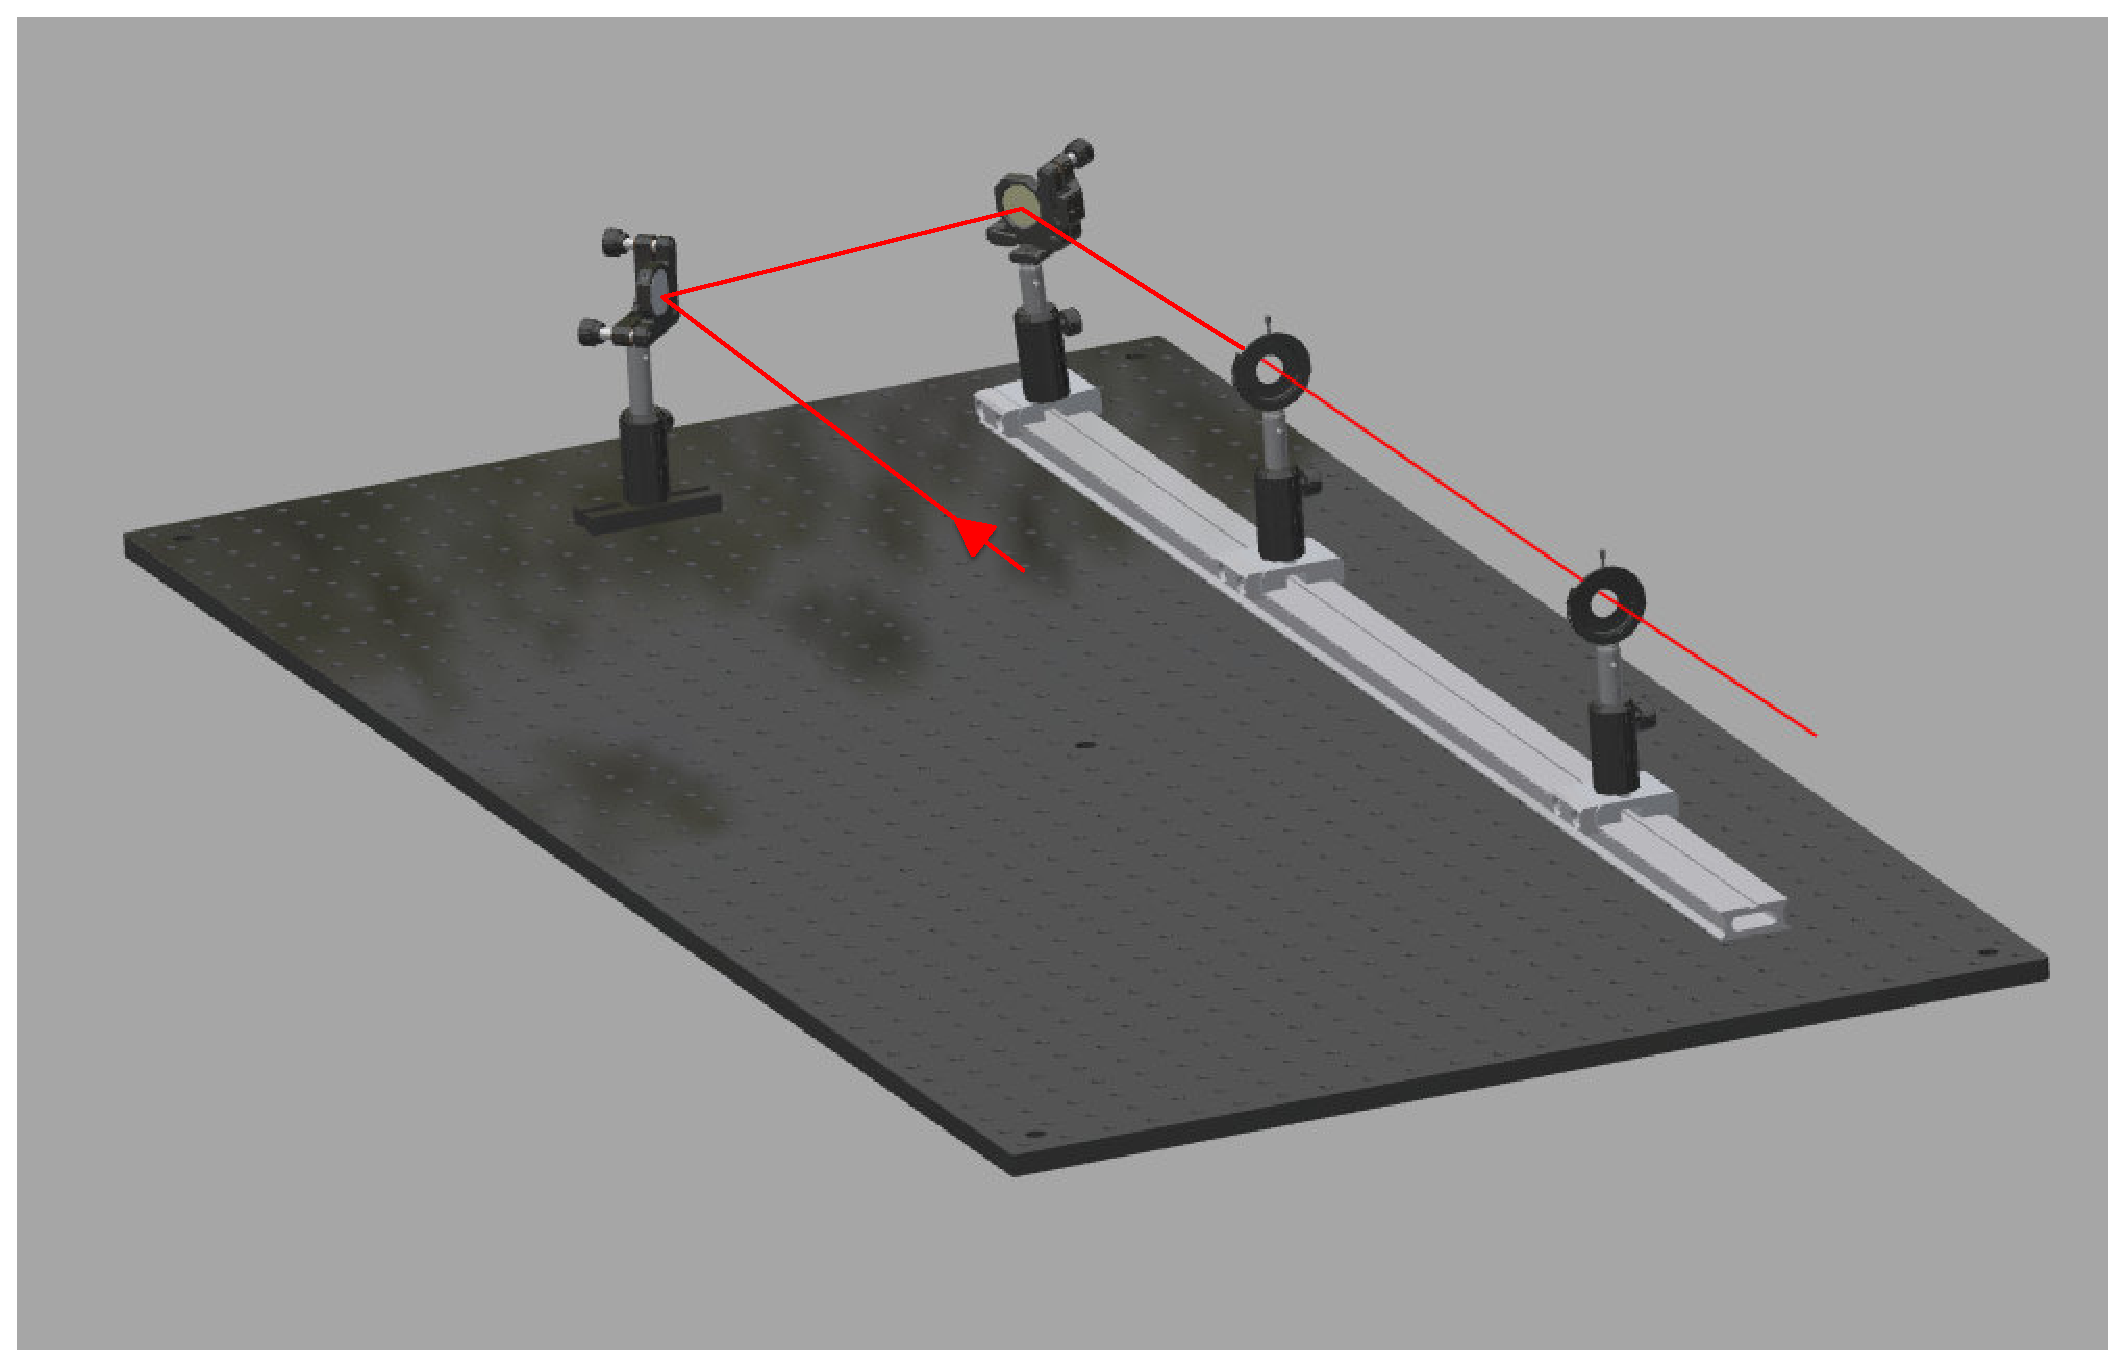
\includegraphics[width=4in]{alignment_CAD_01.eps}
\caption{A beam traveling directly through two irises.}
\label{fig:ex1}
\end{figure}

To understand the procedure you first need to realise that:
\begin{enumerate}
\setlength\itemsep{0.1em}
\item Adjusting the angle of the first mirror \textit{translates} the beam across the surface of the second mirror.
\item Adjusting the angle of the second mirror alters \textit{the angle} with which the beam goes through the irises. 
\end{enumerate}

The irises act as a pair of targets. 
As a consequence of (1), we adjust the first mirror such that the beam passes through the first iris. 
As a consequence of (2), we adjust the second mirror such that the beam passes through the second iris.
We must iterate this procedure because, obviously, the first mirror does not induce pure translation through the system and the second does not induce pure angle change. 
The procedure works because the first mirror induces \emph{relatively} more translation than angle change and the second mirror induces \emph{relatively} more angle change than translation. 
The positioning of the components influences how much iteration is needed.

\clearpage

\subsection{Let's do it!}
Your scanners are installed in a raised cage system with a periscope to bring the beam up from table height (Fig.~\ref{fig:beam_in_cage}. 
You will now need to align the beam such that it enters the bottom periscope mirror, hits the middle of the galvo scan mirrors, then exits travelling along the axis of the cage.
Hints:
\begin{itemize}
    \item The beam should enter square to the periscope and near the middle of of the aperture.
    \item Use the SM2 `T-shirt' target to align the beam along the rail. 
    \item You can look at the scattered light on the galvo mirror surfaces to centre the beam here. 
    \item The galvos must be switched on and at a 0V command voltage (or have the inputs shorted to ground) for the alignment along the cage to be successful. 
\end{itemize}


\begin{figure}[h]
\center
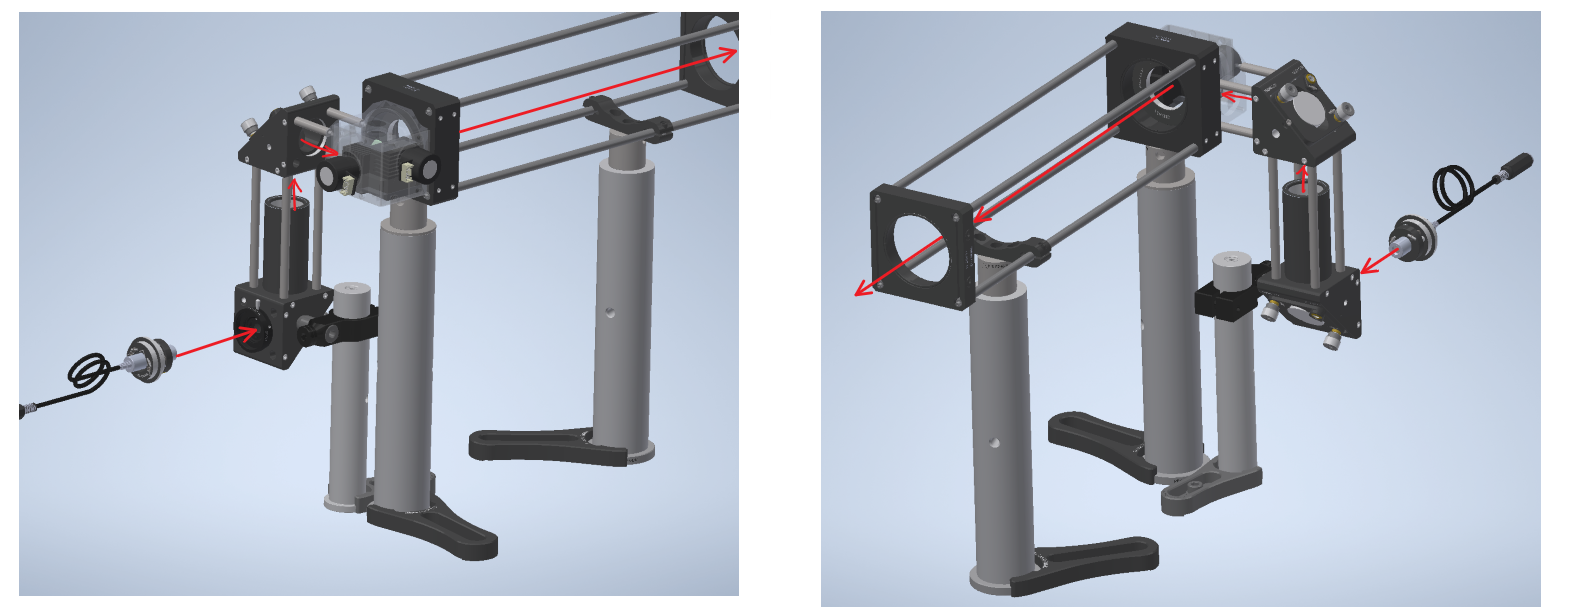
\includegraphics[width=6.5in]{./figures/beam_in_cage.png}
\caption{Scanner cage system shown with laser beam entering periscope and leaving scan box traveling straight down the middle of the cage system. The orientation of your first periscope mirror may differ from that shown here.}
\label{fig:beam_in_cage}
\end{figure}

\clearpage


\section{Driving the scan mirrors}
The two galvos typically move the beam over the sample in a raster pattern.
By convention, the mirror driving the fast axis (along image columns) is known as the $x$ mirror; the mirror driving the slow axis (along image rows) is the $y$ mirror. 
A galvo is a servomotor that allows closed loop control of mirror angle. 
The servo controller accepts a signed analog voltage value which it maps to a mirror angle. 




\subsection{Controlling the scan mirrors}
Measurement \& Automation Explorer (MAX) from NI is used for simple debugging and testing. 
We will explore the basic features of MAX to introduce you to how the mirrors move and confirm the hardware is functioning as expected. 

\begin{itemize}
    \item Open NI MAX
        \begin{enumerate}
            \setlength\itemsep{0.15em}
            \item Select the DAQ device from the list on the left then hit `Test Panels'. 
            \item Select the `Analog Output' tab (Fig.~\ref{DAQMX}).
            \item Set `Mode' to `Voltage Sinewave Generation' and set the amplitude to about `5V'.
            \item Leave the `Rate' at `1000'. This will produce a 1~Hz sine wave because the sample rate is 1~kHz
            \item Connect the analog outputs to the osciloscope and confirm you get waveforms out of both channels. 
        \end{enumerate}

    \item Turn on the laser, copy signals to the scanner controller analog inputs and try driving the scan mirrors with the 1~Hz signal.  Place a card in front of the scanners to visualize the beam. 
    \item Set `Rate' to `50,000' to produce a 50~Hz motion. What does the outgoing beam look like now?
    \item Now try the `DC' option under `Mode'. This sets the analog output line to a single fixed value. Explore how the mirrors respond to this (press `Update' to apply your chosen voltage to the device).
\end{itemize}


\begin{figure}[h]
\centering
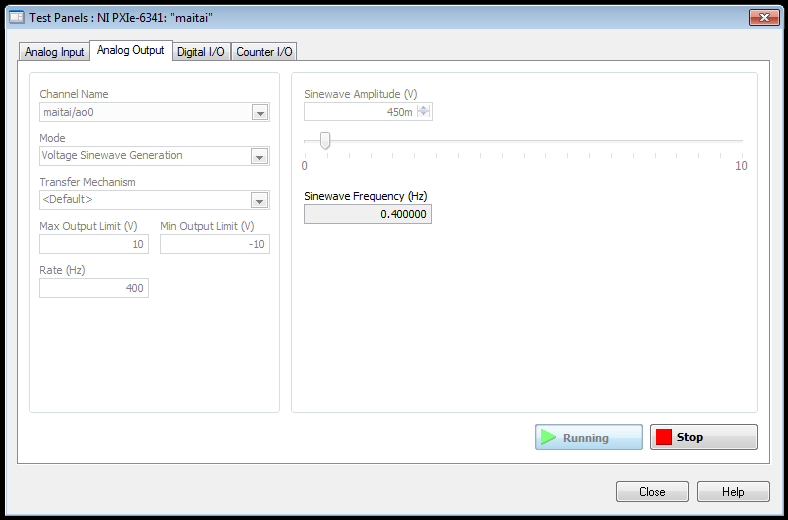
\includegraphics[width=3.5in]{MAX_for_1D.png}
\caption{The NI MAX test panel for analog output.}
\label{DAQMX}
\end{figure}



\clearpage

\section{Building a 1D scan waveform}

You will now use Python to build a 2-D scan pattern. 
First make the following changes to the DAQ breakout box. 

\begin{itemize}
    \setlength\itemsep{0.15em}
    \item Use a BNC T connector to feed the \texttt{AO0} signal to both \texttt{AI0} and the X scanner control box. This will allow us to acquire and monitor the $x$ galvo command signal.
    \item Connect \texttt{AI1} to the galvo position output lead. This will allow us to compare the actual mirror position with the command position.
\end{itemize}

\noindent
The class in \texttt{SimplePyScanner/src/waveformTester.py}\footnote{\textithttps://github.com/SWC-Advanced-Microscopy/SimplePyScanner} generates scan patterns, records the scanner feedback position, and plots the results\footnote{Equivalent code for MATLAB can be found at \textit{https://github.com/SWC-Advanced-Microscopy/SimpleMScanner}, but we will not be using that today.}.  
The scanning code is in \texttt{C:/TEACHING}. 


\begin{itemize}
\setlength\itemsep{0.15em}
\item Fire up an editor and load \texttt{waveformTester.py}. Your machine should have Notepad++ or you can edit in Jupyter.
\item Start an Anaconda command prompt \texttt{cd} to code directory and run \texttt{python waveformTester.py}. 
\item The beam will move and a figure window (below) will appear.
\item The figure window is updating in real time. You can demonstrate this by unplugging and re-plugging the BNC cable going into AO0. 
\item At any time you can stop acquisition and disconnect from the DAQ by pressing return. 
\end{itemize}

\noindent       
With the default scan settings you should see something similar to that shown in Fig.~\ref{waveformTester01}.
The red sinusoid represents the galvo position feedback signal and the white trace represents the command signal. 
The frequency of the waveform is displayed at the command line. 
Right is a position/command phase plot. 
\textbf{Qs. A 0V command voltage asks the scanner to go to its midpoint, sending the beam straight down the cage. Look at the plot. Is this what is happening?}


\begin{figure}[h]
\centering
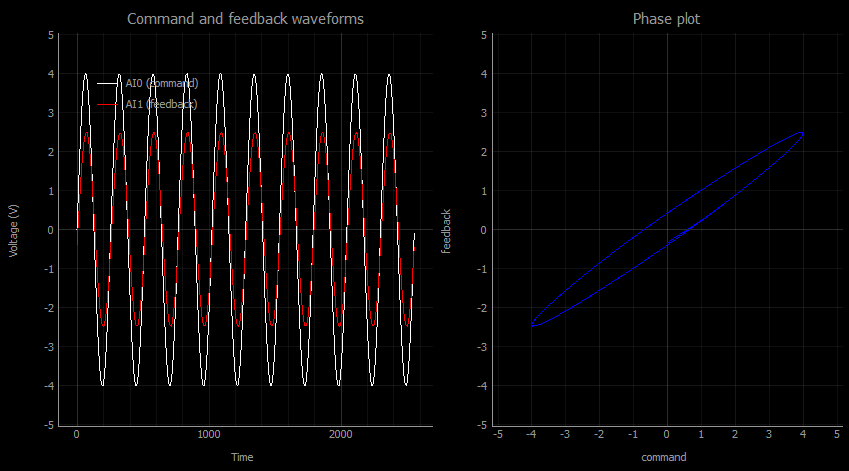
\includegraphics[width=5.0in]{Capture_01.PNG}
\caption{Left: The galvo command signal is shown in white and the feedback signal from the galvo control box is shown in red. 
Right: the feedback signal as a function of the command signal.}
\label{waveformTester01}
\end{figure}


\noindent
Read through the class help text and the code. 
The class has as little extraneous code as possible. 
We use \texttt{pyqtgraph} for plotting because this library excels at generating figures that update rapidly.   
Read through the code and satisfy yourself that you understand how it works. 
Pay particular attention to how the waveform is built in \texttt{generate\_scan\_waveform} and how the DAQ is set up in \texttt{connect\_to\_daq}.
Note how the method \texttt{read\_and\_display\_data} is used as a callback function by \texttt{nidaqmx}. 
Note that:

\begin{itemize}
    \setlength\itemsep{0.15em}
    \item The waveform amplitude is scaled by the \texttt{galvo\_amplitude} attribute.
    \item \texttt{pixels\_per\_line} is the number samples in one cycle of the sine wave. 
    \item The waveform is repeated \texttt{num\_reps\_per\_acq} times, and this many cycles are plotted at once. 
\end{itemize}


\clearpage
\subsection{The effect of command signal frequency}
The scanners have inertia so their ability to follow the command waveform will depend upon its shape and frequency. 
Let's try changing the frequency. 

\begin{itemize}
\item Stop the program (take a screenshot first if you want to compare before and after) and edit the \texttt{sample\_rate} attribute.
Increase it from the default 32E3 to 96E3 (meaning 96,000 $samples/s$). 
(\texttt{sample\_rate} is used by the \texttt{timing.cfg\_samp\_clk\_timing} methods of the AI and AO Tasks to set the sample rate.)
This is done in the \texttt{connect\_to\_daq} method of \texttt{waveformTester}.
\item Re-start \texttt{waveformTester}.
\item Notice the larger phase lag between the position and command and how this is reflected in the phase X/Y plot. 
\end{itemize}

\noindent
Satisfy yourself that you understand why changing \texttt{pixels\_per\_line} also alters mirror frequency. 
e.g. At 96 \texttt{pixels\_per\_line} and $96~kS/s$ sample rate the scanner runs at $1~kHz$. (Don't try running faster than this!)


\subsection{Different waveform types}
Return the sample rate to 32E3 and the number of samples per line to 256. 
Change the \texttt{waveform\_type} attribute from `sine' to `sawtooth' and restart the \texttt{waveformTester}. 
How well is the scanner following the command waveform?
Now try tripling the frequency of the mirror motion: how does it look now?
Satisfy yourself that you understand why the phase plot looks as it does. 

Imagine you are using these waveforms to run the fast scan axis of a confocal. 
What are the advantages and disadvantages of this new waveform for building images?
\emph{Hint}: think about how the beam changes speed during the sawtooth in comparison to the sine wave.
Think also how you might build the image on the PC and how well the mirrors follow the sawtooth waveform.
\vspace{1em}

\section{Building 2D scan waveforms and obtaining an image}

\subsubsection{The Scan Waveforms}
In order to generate an image you will first need to scan the beam with both mirrors such that it forms a raster scan pattern. 
Ensure Analog Output 0 is going to the X mirror command input and Analog Output 1 to the Y mirror command input.
If you wish you can copy these signal to your oscilloscope using BNC T pieces. 

\begin{itemize}
\item Complete the Jupyter notebook at \texttt{exercises/scanwaveforms.ipynb}. 
You should now understand what the X and Y mirror waveforms should look like. 
\item The class \texttt{exercises/scan\_waveform\_output.py} will send these waveforms to the scanners and so generate the scan pattern. 
Complete this class, altering all lines marked \texttt{### EDIT}.
Test it: does the beam move as expected?
\end{itemize}

\subsection{Generating an image from a raster scan}
You will scan the beam over a photodiode and in this way generate a simple image. 
Hook up the output of the photodiode to Analog Input 0 on your DAQ and power up the photodiode.
You will be doing simultaneous AO and AI in order to move the beam and at the same time record light levels (\texttt{waveformTester} also performed simultaneous AO and AI).
The goal is to produce code that achieves the following:

\begin{itemize}
    \item Output two AO waveforms that will together drive the X and Y galvos to scan one frame. 
    \item Simultaneously one AI waveform for this frame will be acquired from the photodiode. 
    \item The AI data will be read off the DAQ buffer at the conclusion of each frame.
    \item The AI data will not, of course, be returned in the form of a 2D array. It will be a series of numbers (a vector) that must be reshaped into a 2D matrix which represents the image.
\end{itemize}

First complete the exercise in Jupyter notebook \texttt{exercises/simpleimage.ipynb}, which demonstrates how a 1D scan waveform is converted into a 2D image. 
\vspace{0.5em}

\noindent
You now have in place all the concepts to run your microscope! 
All that remains is to put them together. 
Complete the \texttt{###EDIT} lines in \texttt{exercises/image\_scanner.py} and run it. 
Once it is running, place the photodiode at the end of the cage system so that the beam passes over it as shown in Fig.~\ref{lineOnPD}.
If it's working you should see a structured image in your figure window.

\begin{itemize}
    \item What does your image look like? Can you explain everything you see? Hints: which axis on the image corresponds with the fast scan direction and how well does the scanner follow the command signal?
    \item Try varying the distance between the detector and the scanners. Is that the same as changing the scan amplitude?
\end{itemize}

\begin{figure}[h]
\centering
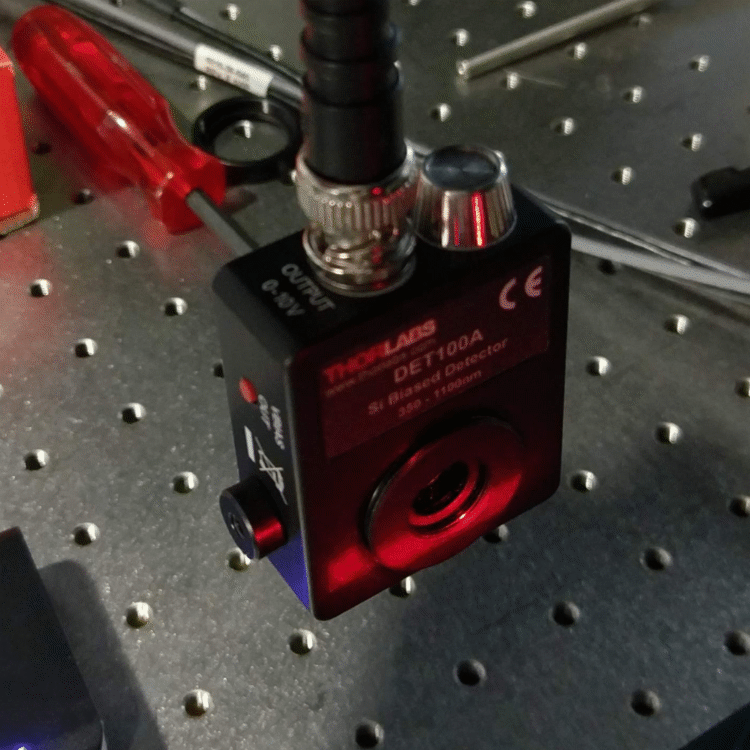
\includegraphics[width=2.0in]{BeamScanningOverPhotoDiode.png}
\caption{The beam scanning over the photodiode. 
         Note that the red laser beam scans over the whole body of the photodiode. 
         The important point is that the beam should not be restricted to the active area of the diode only.}
\label{lineOnPD}
\end{figure}


\clearpage

\section{Imaging with your scanning microscope}
You are now ready to convert your setup into a transmission scanning microscope.
The the sample sits between the laser and the detector, and an image is built up based on the degree to which the sample occludes the scanned beam. 
Choose one of the larger samples in your slide set, like the fly head or the flea, and re-arrange your setup and/or modify the size of the scan pattern to obtain an image. 
Do you get an image of the sample? 
Are you happy with the image?
Take a screenshot of your best attempt.
\vspace{0.5em}

\noindent
There is an optical element you can add to the path that will lead to a radically better image. 
What is that element and where should it go? Try it. 
Take a screenshot of your best attempt.




\section{The scan engine}
At this point you should have obtained a pretty decent image of your sample, but you can do better!
Estimate the resolution of your microscope using Abbe's criterion. 
What specification do you need to change in your microscope to improve the resolution?
\emph{Hint}: A thin beam enters and leaves the scanners but we want a larger beam to be pivoting at the objective back aperture  (Fig.~\ref{pivot}).
Modify your microscope to achieve this and re-image your sample.


\begin{figure}[h]
\centering
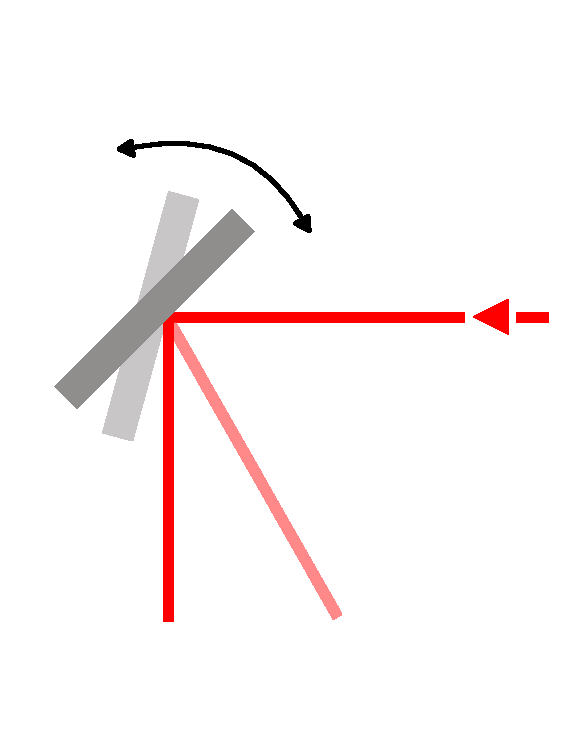
\includegraphics[width=1.2in]{ScanMirrorBeam.eps}
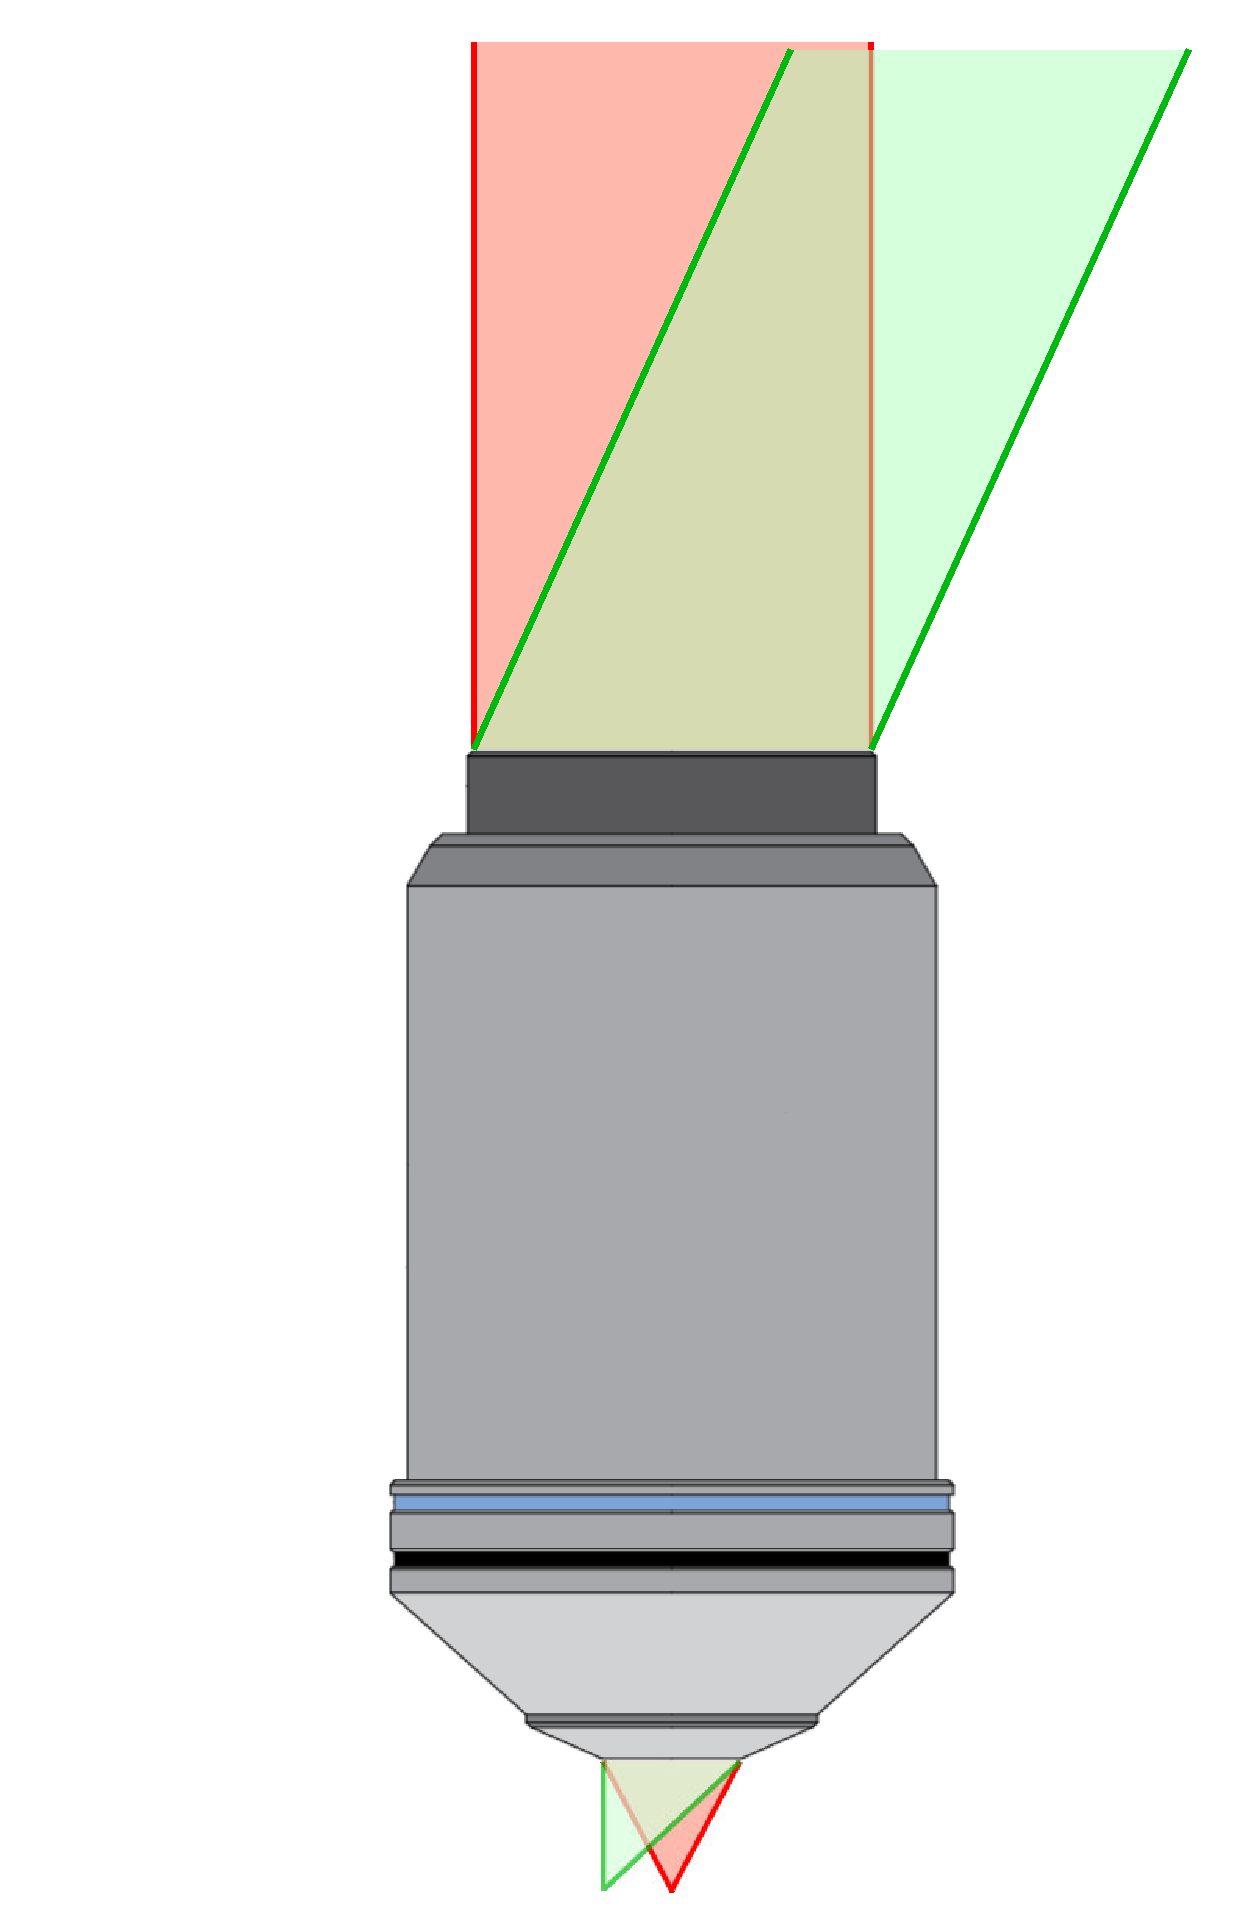
\includegraphics[width=1.2in]{Objective_pivot.eps}
\caption{Left: A scan mirror deflects a laser beam as it pivots about its axis.
Right: In order to scan a focused spot across a sample, the beam must pivot at the back aperture of the objective. }
\label{pivot}
\end{figure}

\section{Bonus Exercises: The code and the scan pattern}
We built images based on the command waveforms. 
In other words, we assume the beam is located where we asked it to be and we placed the pixels at that location.
Since the actual beam position does not follow the expected position, this produces artifacts. 
Which part of the fast scan pattern is most responsible for the artifact?
There is a waveform that would minimize the artifact and allow the scanners to run faster. What is it? Try building this and obtaining an image with it. 

Alternatively, look at \texttt{basicScanner.py} and the \texttt{set\_amplitude} method. Try adding a method to change the image size on the fly. 

\end{document}
